
\section{Codifica}
\subsection*{Librerie e \textit{framework} utilizzati}
\subsubsection*{Jersey}
Per la creazione servizi \textit{REST}, ho utilizzato Jersey che, tramite annotazioni su metodi e classi, 
mi ha permesso di creare facilmente i vari servizi.
Il frammento di codice \ref*{lst:rest-service} mostra un esempio di \textit{servizio REST} che restituisce tutte le dipendenze di un pacchetto.\\
\begin{lstlisting}[language=Java, caption={Esempio di \textit{servizio REST} utilizzando Jersey.},captionpos=b, label={lst:rest-service}]
  @GET ()
  @Path ("dependency/byPackage/{id}")
  @Produces (MediaType.APPLICATION_JSON) @Consumes (MediaType.APPLICATION_JSON)
  public Response byPackage (@PathParam ("id") String id, 
        @QueryParam ("withDev") boolean withDev, 
        @QueryParam ("withCompile") boolean withCompile, 
        @QueryParam ("withRuntime") boolean withRuntime
  ) {
      return Response.ok (DependencyLogic.get ().getDependenciesByPackage (id, withDev, withCompile, withRuntime)).build ();
  }
\end{lstlisting}

\subsubsection*{Neo4j}
Per la gestione del \textit{database} Neo4j, ho utilizzato la libreria \textbf{Neo4j Java Driver}, 
che mette a disposizione una serie di classi e metodi per l'apertura e la gestione delle connessioni al \textit{database} e 
per l'esecuzione di \textit{query} Cypher.\\

\subsubsection*{Smi-commons}
Per la gestione delle operazioni comuni, come la gestione del \textit{logger}, la gestione delle eccezioni, la lettura dei 
file di configurazione e la gestione del \textit{token}, ho utilizzato una libreria sviluppata da \azienda{}, denominata \textit{smi-commons}.\\

\subsubsection*{Nx}
Per la creazione e gestione del progetto Angular, ho utilizzato il \textit{tool} \textbf{Nx}, 
che permette di creare progetti Angular senza dover pensare alla struttura del progetto.\\
Nx mette a disposizione una serie di comandi per la creazione di progetti, moduli, componenti, servizi e librerie,
e permette di eseguire i \textit{test} e il \textit{build} del progetto.\\
Nx viene utilizzato principalmente per la gestione di progetti \textit{monorepo}, ovvero progetti che contengono più applicazioni,
in modo da poter condividere le librerie tra le varie applicazioni.\\
Nel mio caso però avevo solo un'applicazione, ma ho deciso di utilizzarlo comunque per sfruttare le semplificazioni sulla gestione 
dei \textit{test} e del \textit{build} della progetto.\\

\subsection*{Interrogazioni su \textit{database} a grafo}
Per la gestione delle interrogazioni su \textit{database} a grafo, ho utilizzato il linguaggio Cypher,
che è un linguaggio dichiarativo per la manipolazione di grafi.\\
Questa è stata la parte più complessa del progetto, in quanto non avevo mai utilizzato un \textit{database} a grafo,
e non conoscevo il linguaggio Cypher.\\
Per imparare il linguaggio, ho seguito un corso sulla piattaforma \textbf{Udemy}, messa a disposizione da \azienda{},
che mi ha permesso di apprendere le basi del linguaggio.\\

\subsubsection*{Cypher}
Cypher è il linguaggio di query utilizzato da Neo4j. La sua sintassi è stata progettata per essere intuitiva e leggibile, 
facilitando l'interazione con i grafi. Di seguito, alcuni aspetti chiave della sintassi di Cypher:

\begin{itemize}
\item \textbf{Nodi e Relazioni}: In Cypher, i nodi sono rappresentati da parentesi tonde (es. \texttt{(nodo)}), 
mentre le relazioni sono indicate da frecce con parentesi quadre (es. \texttt{-[relazione]->}). Questa rappresentazione visiva è coerente con la struttura dati del grafo.

\item \textbf{\textit{Pattern Matching}}: Un elemento fondamentale di Cypher è il pattern matching. 
Ad esempio, la query \texttt{MATCH (a)-[r]->(b)} trova tutti i nodi \texttt{a} che hanno una relazione \texttt{r} con i nodi \texttt{b}, permettendo di navigare e interrogare efficacemente i grafi.

\item \textbf{Filtraggio}: È possibile filtrare i risultati utilizzando la clausola \texttt{WHERE}. 
Per esempio, \texttt{MATCH (n) WHERE n.name = 'Alice' RETURN n} restituisce tutti i nodi dove il nome è Alice.

\item \textbf{Creazione e Modifica}: Cypher permette anche di creare e modificare i grafi. 
Le clausole \texttt{CREATE} e \texttt{MERGE} sono utilizzate per aggiungere nodi e relazioni, mentre \texttt{SET} e \texttt{REMOVE} servono per modificare o rimuovere proprietà.

\item \textbf{Aggregazione e Ordinamento}: Cypher supporta operazioni di aggregazione come \texttt{COUNT}, \texttt{SUM}, 
\texttt{AVG}, e permette l'ordinamento dei risultati con \texttt{ORDER BY}.
\end{itemize}

Queste caratteristiche rendono Cypher un linguaggio potente e flessibile per lavorare con i dati in Neo4j, 
facilitando la rappresentazione e l'analisi di relazioni complesse in un formato di grafo.\\

Con la query mostrata nel frammento di codice \ref*{fig:query-cipher} carico tutti i nodi che hanno un collegamento di tipo \textbf{D} o \textbf{R} con il nodo di partenza,
e per ogni nodo carico tutti i nodi collegati ad esso.\\
Questa \textit{query} viene utilizzata per caricare in modo \textit{lazy} l'albero delle dipendenze, ovvero carico solo i nodi che sono direttamente collegati al nodo di partenza,
e calcolo il numero di figli per ogni nodo.\\ In questo modo posso mostrare un \textit{badge} su ogni nodo con il numero di figli, e posso caricare i figli solo quando l'utente espande il nodo, 
vedi la figura \ref{fig:frontend-4-bis}.\\

\begin{figure}[h]
  \centering
  \begin{minipage}{0.550\textwidth}
      \centering
      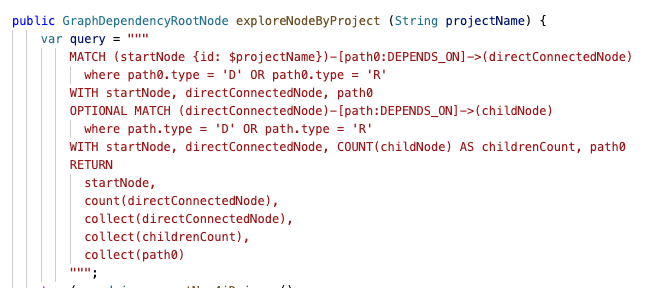
\includegraphics[width=\textwidth]{query-cipher} 
      \caption{Esempio di \textit{query} Cypher per l'esplorazione dell'albero delle dipendenze.}
      \label{fig:query-cipher}
  \end{minipage}\hfill
  \begin{minipage}{0.450\textwidth}
    \centering
    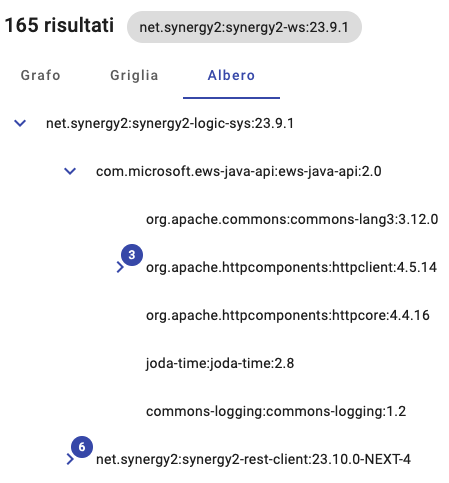
\includegraphics[width=.6\textwidth]{frontend-4}
    \caption{Risultato query \ref*{fig:query-cipher}.}
    \label{fig:frontend-4-bis}
  \end{minipage}
\end{figure}

\subsection*{Ricerca di aggiornamenti e vulnerabilità}
Per la ricerca di aggiornamenti delle dipendenze, ho utilizzato i servizi gratuiti offerti da \textbf{OSS Index},
che permettono di verificare se una dipendenza è aggiornata o meno.\\
Effettuando, ad esempio, la seguente chiamata \textit{GET} \textit{REST} al servizio \\
% use small text inside lstlisting
\begin{lstlisting}[language=Java, caption={Esempio di chiamata al servizio \textbf{OSS Index} per la ricerca di aggiornamenti.},captionpos=b, label={lst:oss-index}
  ,basicstyle=\small]
  https://search.maven.org/solrsearch/select?q=g:com.google.code.gson+a:gson
\end{lstlisting}
avremo come risultato un \textit{JSON} contenente una serie di informazioni riguardanti il pacchetto, tra cui
l'ultima versione disponibile.\\

Questa chiamata viene effettuata per ogni dipendenza del progetto selezionato, e viene confrontata con la versione utilizzata nel progetto.\\
In caso di aggiornamento, viene stampato un messaggio di avviso, come mostrato nella figura \ref{fig:frontend-8}.\\

Per la ricerca di vulnerabilità, ho utilizzato il servizio \textbf{OWASP Dependency-Check}, che permette di verificare se una dipendenza
ha delle vulnerabilità.\\
Anche in questo caso vengono raccolti i risultati per ogni dipendenza, e in caso di vulnerabilità viene stampato un messaggio di avviso.